\documentclass[a4,12pt]{article}

\usepackage[francais]{babel}
\usepackage[utf8]{inputenc}
\usepackage[T1]{fontenc}
\usepackage[babel=true]{csquotes}
\usepackage{amsmath}
\usepackage{amssymb}
\usepackage{float}
\usepackage{graphicx}
\usepackage{wrapfig}
\usepackage{hyperref}
\usepackage{array,multirow,makecell}
\frenchbsetup{StandardLists=true}
\usepackage{enumitem}
\setlength\parindent{20pt}
%\graphicspath{{/Documents/2A/Semestre1/Projet_GL/docs/}}
\begin{document}
\begin{titlepage}
\title{ Documentation technique sur la classe Math.}
\author{Fischman Adrien, Geoffroy Germain.}
\date{}

\maketitle

\rule[0.5ex]{\textwidth}{0.2mm}
Ce document a pour but d'expliquer la conception de la classe Math.decah.\\
Il présente à la fois les algorithmes utilisés, ainsi que les choix mathématiques et informatiques nécessaires à l'implémentation, mais aussi la démarche qui a permis d'aboutir.\\
La validation et les limites de nos algorithmes sont décrites au fur et à mesure, expliquant les choix que nous avons étés amenés a prendre.

\rule[0.5ex]{\textwidth}{0.2mm}

\end{titlepage}
\tableofcontents
\newpage
\section{Introduction.}
La classe Math contient différentes méthodes :
\begin{itemize}
    \item float ulp(float f)
    \item float sin(float f)
    \item float cos(float f)
    \item float asin(float f)
    \item float atan(float f)
\end{itemize}
L'implémentation de ces différentes méthodes se doit donc de minimiser les sources d'imprécisions, qui proviennent d'une part des approximations mathématiques nécessaires aux algorithmes utilisés mais aussi des limites de précision liées à la représentation des nombres flottants simple précision, afin d'atteindre la meilleur approximation possible des ces différentes fonctions mathématiques.
\subsection{Nombre flottant simple précision.}
La représentation des nombres flottants simple précision se fait en un mot de longueur 32 bits avec : un bit de signe, 8 bits pour l'exposant et 23 bits pour la mantisse.\\
Un nombre flottant normalisé (ie dont l'exposant décalé est différent de 0 et de 127 et que le bit de poids fort de la mantisse est 1) est de valeur $x$ est donné par : \\
$$ x = s.2^{e}.m\ ,\ avec
 \left \{
	\begin{array}{l}
	s = \pm 1\ repr\acute esente\ le\ signe (selon\ le\ bit\ de\ signe)\\
	e\ est\ l'exposant\ avant\ son\ d\acute ecalage\ de\ 127\\
	m = 1 + mantisse,\ repr\acute esente\ la\ partie\ significative\ (en\ binaire)\\
	\end{array}
\right.
$$
\begin{figure}[b]
    \centering
    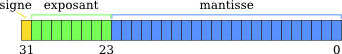
\includegraphics{float.png}
    \caption{Nombres flottants simple précision.}
    \label{Représentation des nombres flottants simple précision.}
\end{figure}

\subsection{Mesure de l'approximation.}
Afin de mesurer l'approximation faite par nos calculs, nous utilisons l'unité de précision élémentaire sur les nombres flottants : ULP (Unit in the Last Place). L'ULP d'une flottant f représente la distance en nombre flottant entre f et le flottant le plus proche de f.\\
Ainsi la précision des calculs se mesure en ULP. Lorsque que l'on approche un nombre $x$ par le nombre approximé $\tilde x$, on mesure $ \frac{ulp(x - \tilde x)}{ulp(x)} $ pour exprimer l'écart entre la valeur approchée et la valeur exacte.

\subsection{Validation des algorithmes.}
Pour confronter nos résultats avec les valeurs mathématiques attendues, nous utilisons les fonctions prédéfinies de Java. On compare alors nos valeurs à celle retournée par Java ce qui implique donc que la validation de nos résultats ne constitue qu'une seconde approximation de la valeur mathématique.\\
Cependant, en pratique, atteindre un niveau de précision de quelques ULP est suffisant pour notre implémentation et c'est l'objectif que nous nous sommes fixé.
\section{Fonction ulp.}
\section{Fonction sin et cos.}
\subsection{Algorithme de Cordic.}
\subsection{Développement en série entière.}

\begin{tabular}{|c|c|c|c|c|c|}

\hline 
 & intervalle & nombre d'erreur($ > 1 ulp$) & erreur max(ulp) & pas & nombres de tests \\
\hline 
sin & $[0;\pi /4]$ & 229 & $2$ & $2^{-17}$ & 102944\\
\hline
sin & $[\pi /4;\pi /2]$ & 985 & $3$ & $2^{-17}$ & 102944\\
\hline
sin & $[\pi /2;\pi .3/2]$ & 5761 & $3$ & $2^{-17}$ & 411775\\
\hline
\end{tabular}

\begin{tabular}{|c|c|c|c|c|c|}

\hline 
 & intervalle & nombre d'erreur($ >  ulp$) & erreur max(ulp) & pas & nombres de tests \\
\hline
cos & $[0;\pi /8]$ & 3(>1ulp) & $2$ & $2^{-17}$ & 51472\\
\hline
cos & $[\pi /8;\pi /4]$ & 4544(>1ulp) & $2$ & $2^{-20}$ & 411775\\
\hline
cos & $[\pi /4;3\pi /8]$ & 5771(>1ulp) & $2$ & $2^{-20}$ & 411775\\
\hline
cos & $[3\pi /8;\pi /2]$ & 2166(>1ulp) & $2$ & $2^{-20}$ & 411775\\
\hline
cos & $[\pi /2;\pi .1.005/2]$ & 1025(>50ulp) & $1.2303662E7$ & $2^{-17}$ & 1030\\
\hline
cos & $[\pi /2;5\pi /8]$ & 316165 & 279598 & $2^{-20}$ & 411775\\
\hline
\end{tabular}


\subsection{Algorithme de Cody and Waite}
\section{Fonction asin.}
\section{Fonction atan.}
\end{document}